\section{Results}
\label{sec:results}

\subsection{Steering Influence Decays Within One Token}

\Figref{fig:main_decay} shows the $\deltaprojection$ curves for all steering conditions. During the steered window (shaded), the projection reaches values of 12--29 depending on condition. The moment the steering vector is removed, $\deltaprojection$ drops precipitously. Within one token, the signal falls to less than 5\% of its peak value across all conditions.

\begin{figure}[t]
\centering
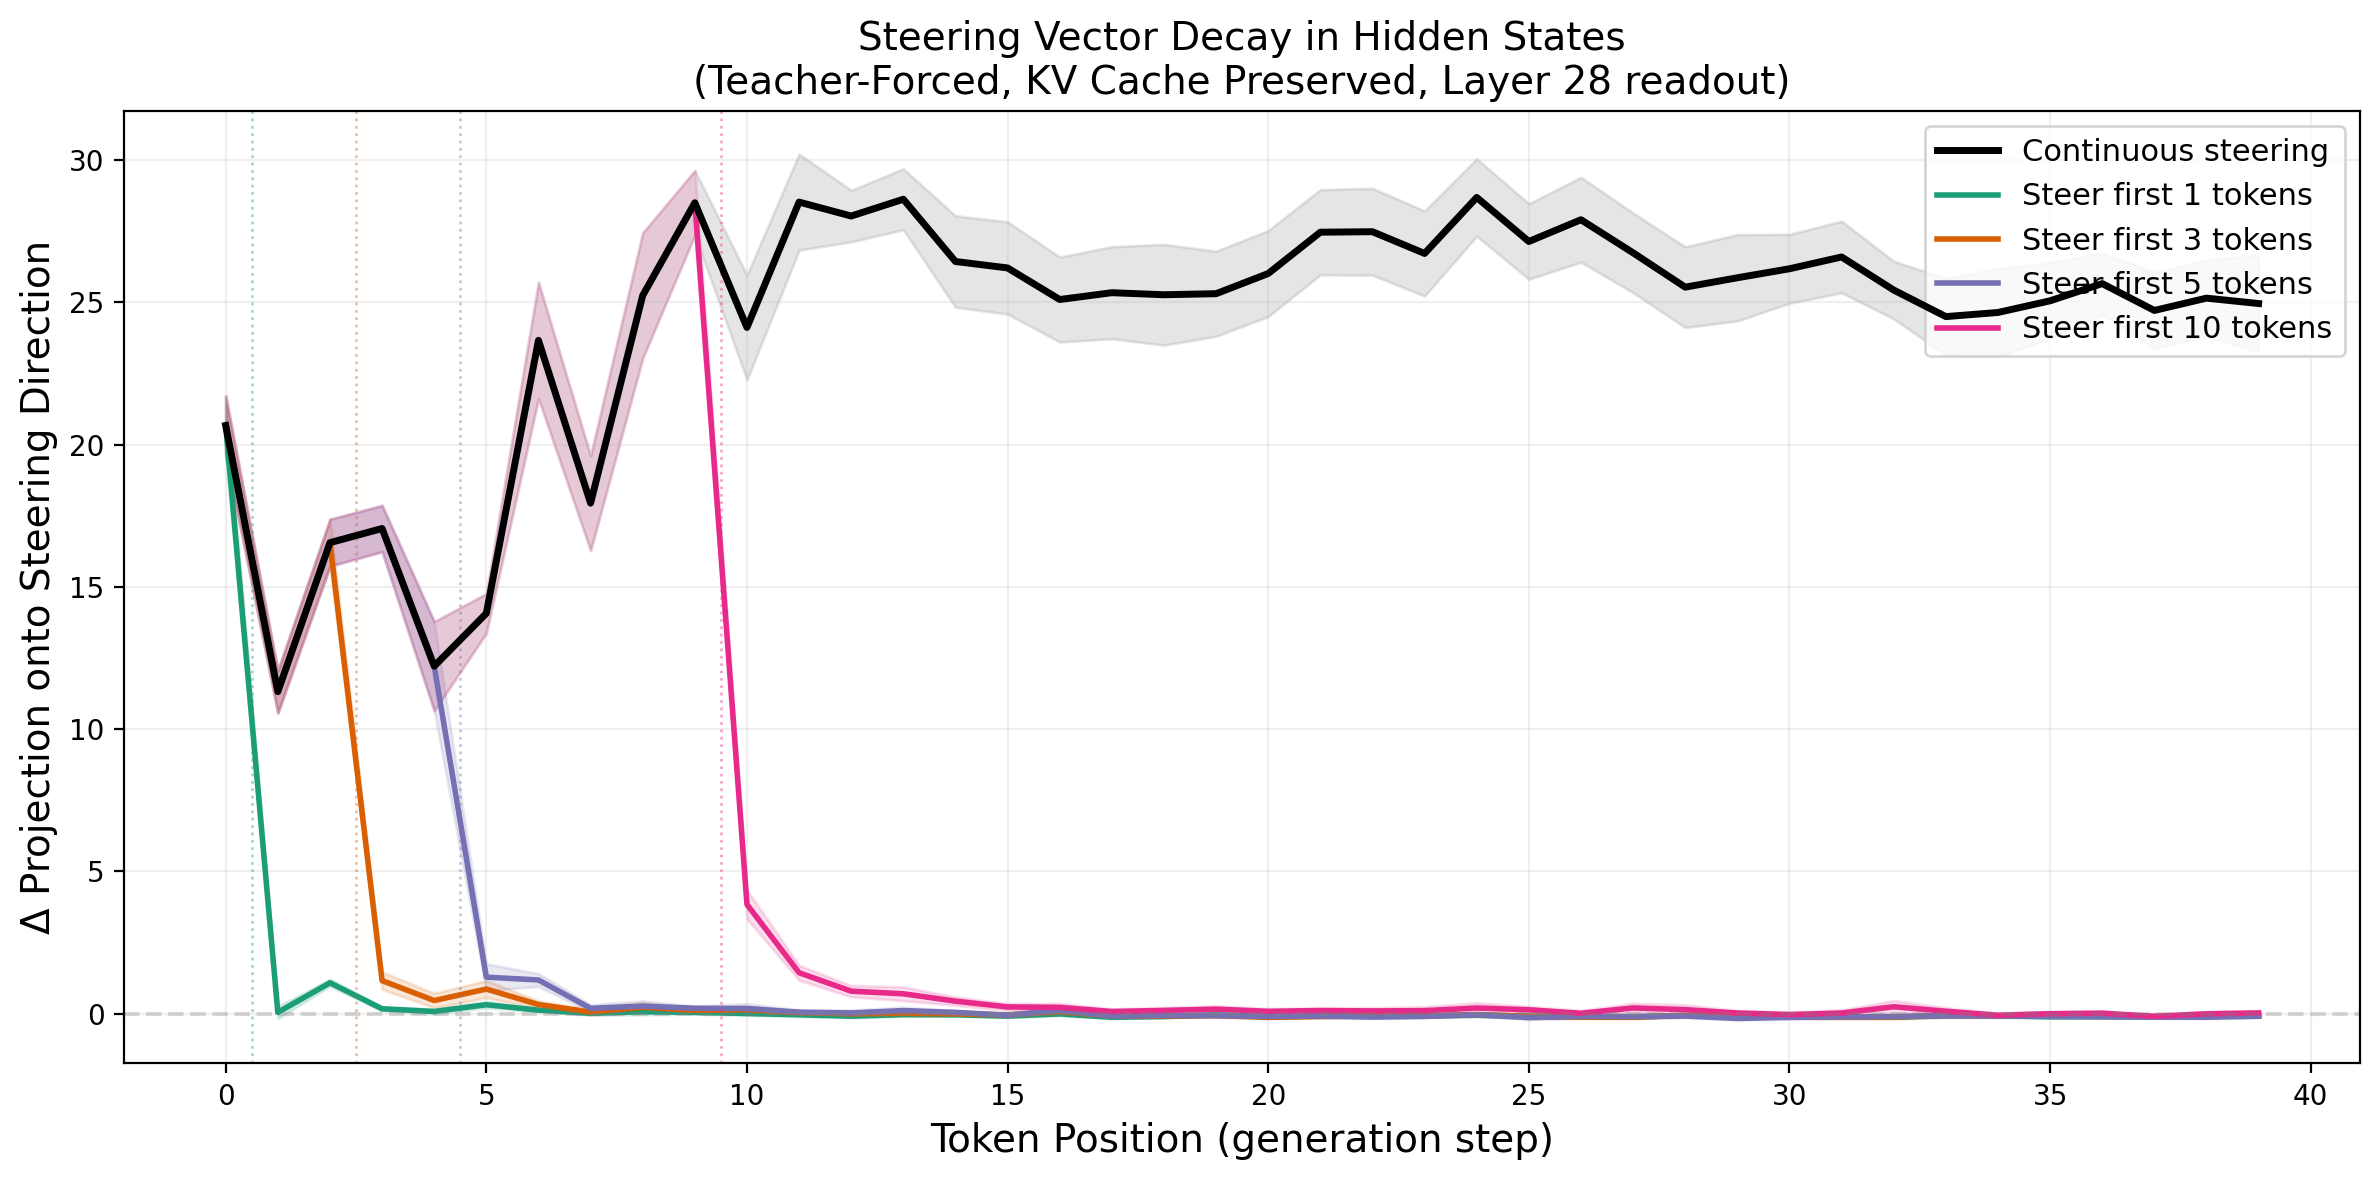
\includegraphics[width=0.95\linewidth]{figures/fig1_main_decay.png}
\caption{Steering influence ($\deltaprojection$) over generation steps. The steering vector is applied for the first $N$ steps (shaded region), then removed. Under all initial-steering conditions (with KV cache preserved), the perturbation drops to near-zero within 1--2 tokens after removal. Continuous steering (gray dashed) maintains $\deltaprojection \approx 24$ throughout.}
\label{fig:main_decay}
\end{figure}

\Tabref{tab:decay} quantifies this decay. The post-steering residual (averaged over 5 steps after removal) ranges from 1.7\% of peak ($N = 1$) to 5.1\% ($N = 5, 10$). Even the largest residual (1.45 for $N = 10$) is small compared to the continuous-steering mean of 24.31.

\begin{table}[t]
\centering
\caption{Steering decay statistics across initial-steering conditions (teacher-forced, KV cache preserved). Peak $\deltaprojection$ is the maximum value during steering. Post-5 and Post-10 averages are computed over the 5 and 10 steps immediately after steering stops. Best (slowest) decay highlighted in \textbf{bold}.}
\label{tab:decay}
\begin{tabular}{@{}lccccccc@{}}
\toprule
$N$ & Peak $\deltaprojection$ & Post-5 avg & Post-10 avg & \% of peak & $\timeconstant$ (tokens) & $R^2$ \\
\midrule
1  & 20.67 & 0.34 & 0.20 & 1.7\% & \textbf{5.82} & 0.506 \\
3  & 16.55 & 0.58 & 0.34 & 3.5\% & 3.35 & 0.889 \\
5  & 12.21 & 0.63 & 0.36 & \textbf{5.1\%} & 2.42 & 0.905 \\
10 & 28.50 & \textbf{1.45} & \textbf{0.81} & \textbf{5.1\%} & 1.21 & \textbf{0.974} \\
\midrule
Continuous & 24.31 (mean) & --- & --- & 100\% & --- & --- \\
\bottomrule
\end{tabular}
\end{table}

\subsection{Exponential Decay Fits}

\Figref{fig:decay_fits} shows the exponential fits to post-steering $\deltaprojection$ values. The fit quality improves with more steered tokens: $R^2 = 0.51$ for $N = 1$ (barely any post-steering signal to fit) and $R^2 = 0.97$ for $N = 10$. The time constants decrease with $N$: $\timeconstant = 5.82$ tokens for $N = 1$ down to $\timeconstant = 1.21$ tokens for $N = 10$.

\begin{figure}[t]
\centering
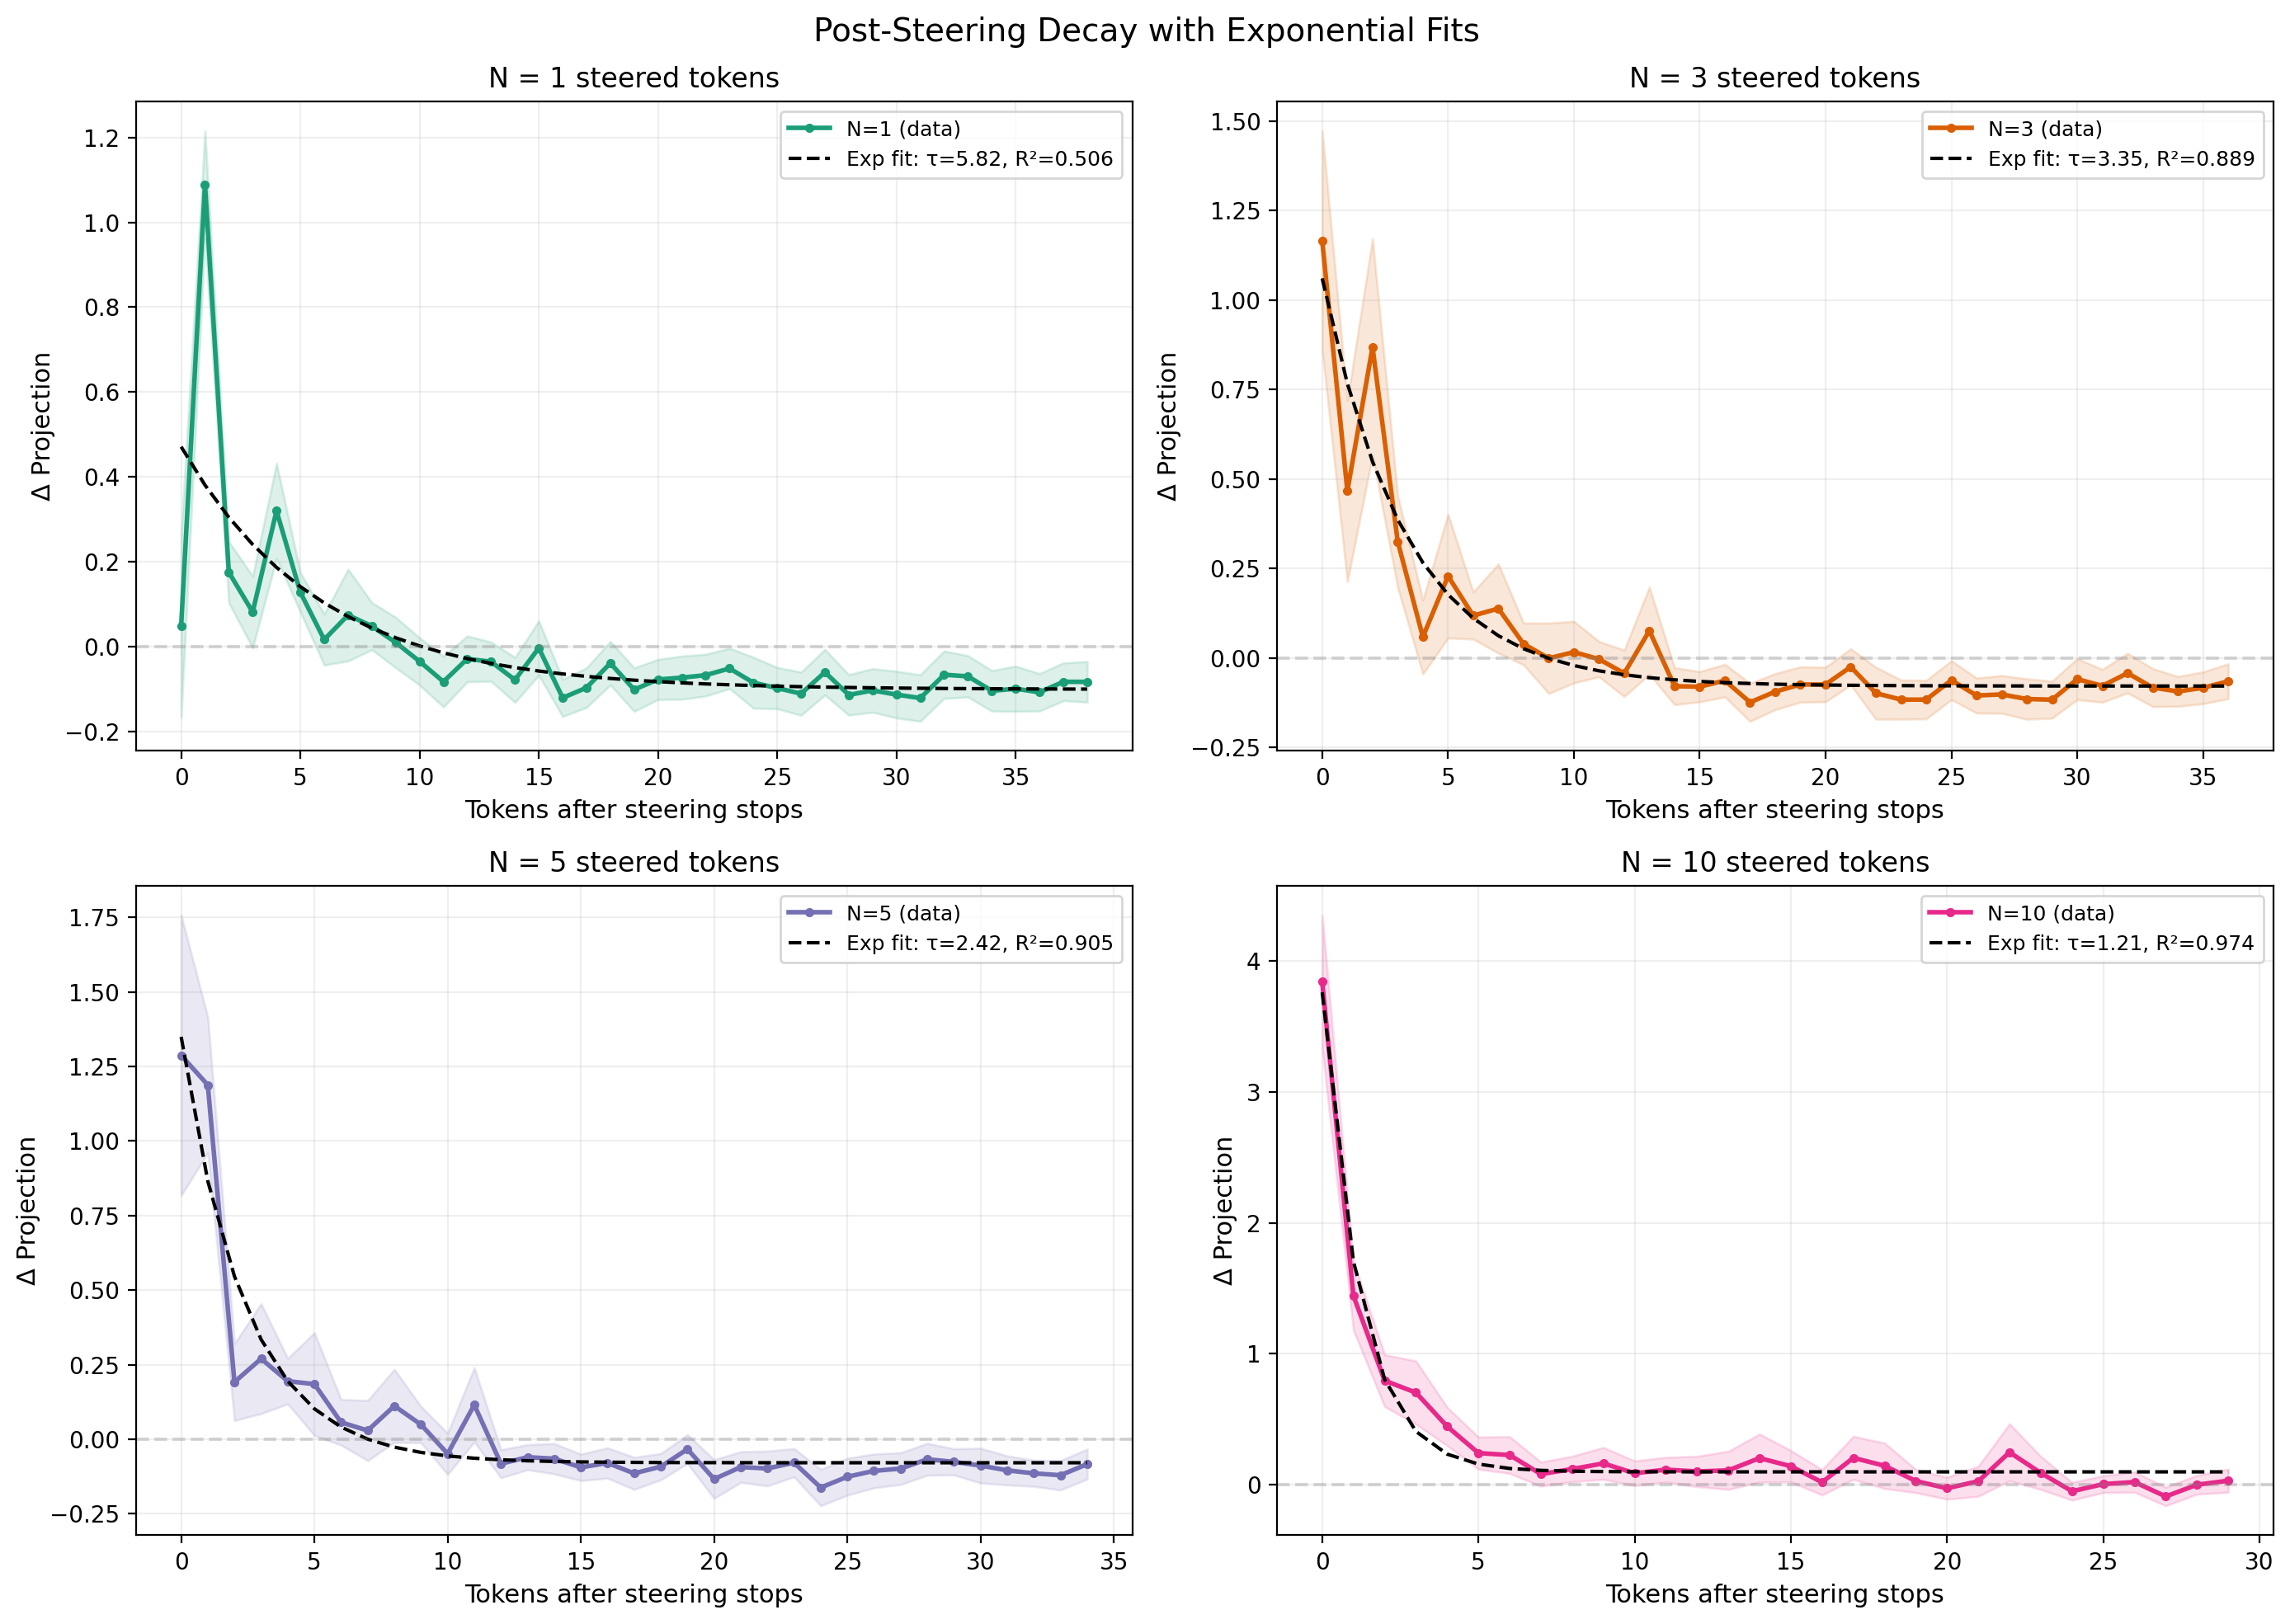
\includegraphics[width=0.95\linewidth]{figures/fig2_decay_fits.png}
\caption{Exponential decay fits (Eq.~\ref{eq:decay}) to post-steering $\deltaprojection$ values. Solid lines show observed means across 60 prompts; dashed lines show fitted curves. The time constant $\timeconstant$ decreases with more initial steering tokens, indicating that larger perturbations trigger faster corrective dynamics.}
\label{fig:decay_fits}
\end{figure}

This inverse relationship between $N$ and $\timeconstant$ is counterintuitive: one might expect more steering to produce slower decay, but instead the model corrects faster. In absolute terms, $N = 10$ does produce a higher residual (1.45 vs.\ 0.34 for $N = 1$), but relative to its much larger peak, the decay is faster.

\subsection{KV Cache Is the Primary Persistence Mechanism}

\Figref{fig:kv_cache} compares the Initial-$N$ condition (KV cache preserved) with the Initial-$N$-NoCache condition (KV cache reset after steering). The results reveal a striking asymmetry:

\begin{itemize}[leftmargin=*,itemsep=0pt,topsep=0pt]
\item \textbf{With KV cache}: $\deltaprojection$ stays slightly positive after steering stops, indicating a small residual alignment with the steering direction.
\item \textbf{Without KV cache}: $\deltaprojection$ goes \emph{negative}, meaning the model's hidden states are pushed \emph{away} from the steering direction relative to baseline---an overcorrection.
\end{itemize}

\begin{figure}[t]
\centering
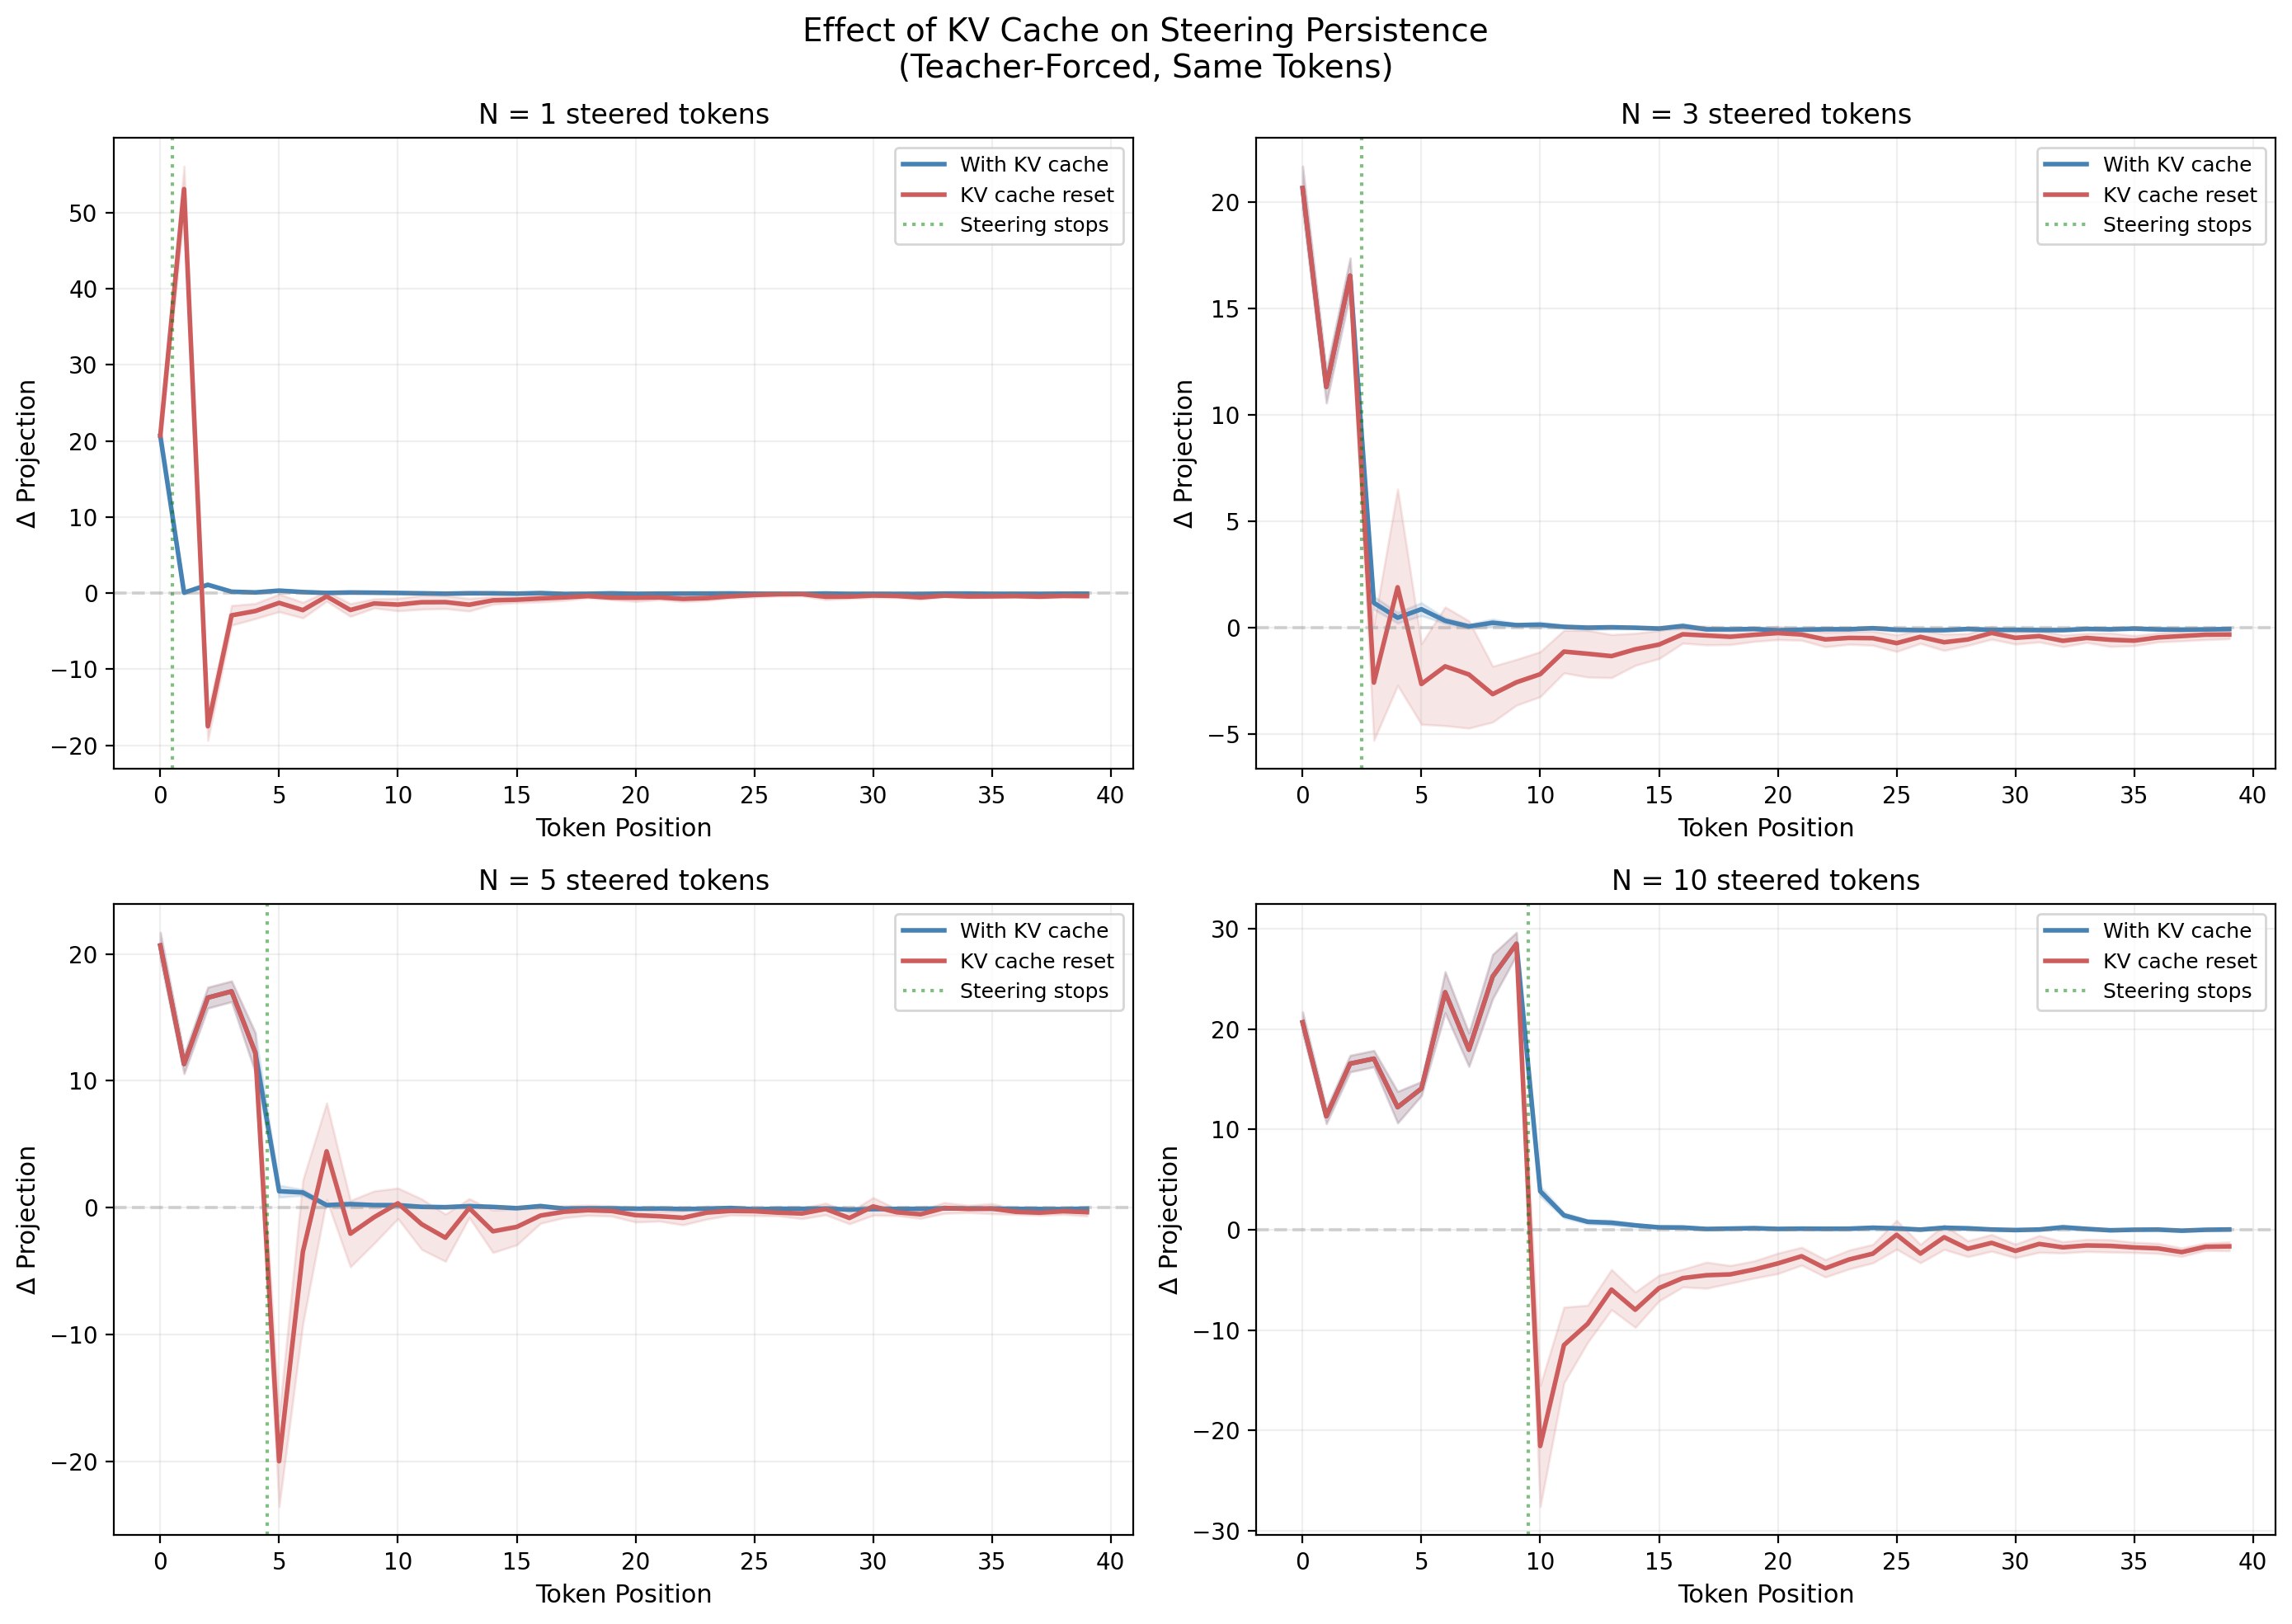
\includegraphics[width=0.95\linewidth]{figures/fig3_kv_cache_effect.png}
\caption{KV cache effect on steering persistence. \figtop: Initial-$N$ with KV cache preserved shows a small positive residual after steering stops. \figbottom: Resetting the KV cache at step $N$ produces a negative rebound (overcorrection), indicating the model adapts to the presence of steered attention patterns.}
\label{fig:kv_cache}
\end{figure}

\Tabref{tab:kv_cache} reports the paired $t$-test results. The difference is statistically significant for all $N$ values ($p < 0.01$), with effect sizes ranging from moderate ($d = 0.53$ for $N = 3$) to very large ($d = 3.41$ for $N = 10$). The negative $t$-statistic for $N = 1$ indicates that even a single steered KV pair, when removed, causes the model to overcorrect more strongly than with the cache preserved.

\begin{table}[t]
\centering
\caption{Paired $t$-test comparing post-steering $\deltaprojection$ (averaged over 10 steps) between KV-cache-preserved and KV-cache-reset conditions across 60 prompts. Positive Cohen's $d$ indicates the KV cache preserves a more positive (steering-aligned) residual.}
\label{tab:kv_cache}
\begin{tabular}{@{}lcccc@{}}
\toprule
$N$ & $t$-statistic & $p$-value & Cohen's $d$ & Interpretation \\
\midrule
1  & $-5.22$ & $< 0.0001$ & $-0.98$ & Cache reset $\Rightarrow$ overcorrection \\
3  & $2.75$  & $0.008$    & $0.53$  & KV cache preserves positive residual \\
5  & $3.74$  & $0.0004$   & $0.74$  & Strong KV cache effect \\
10 & $17.83$ & $< 0.0001$ & $\mathbf{3.41}$ & Very large KV cache effect \\
\bottomrule
\end{tabular}
\end{table}

\subsection{Normalized Decay Curves}

\Figref{fig:normalized} shows all conditions normalized to their peak value. Regardless of $N$, all curves drop below 10\% of peak within 1--3 tokens after the steering vector is removed. This confirms that the rapid decay is a robust property of the system, not an artifact of particular $N$ values or absolute magnitudes.

\begin{figure}[t]
\centering
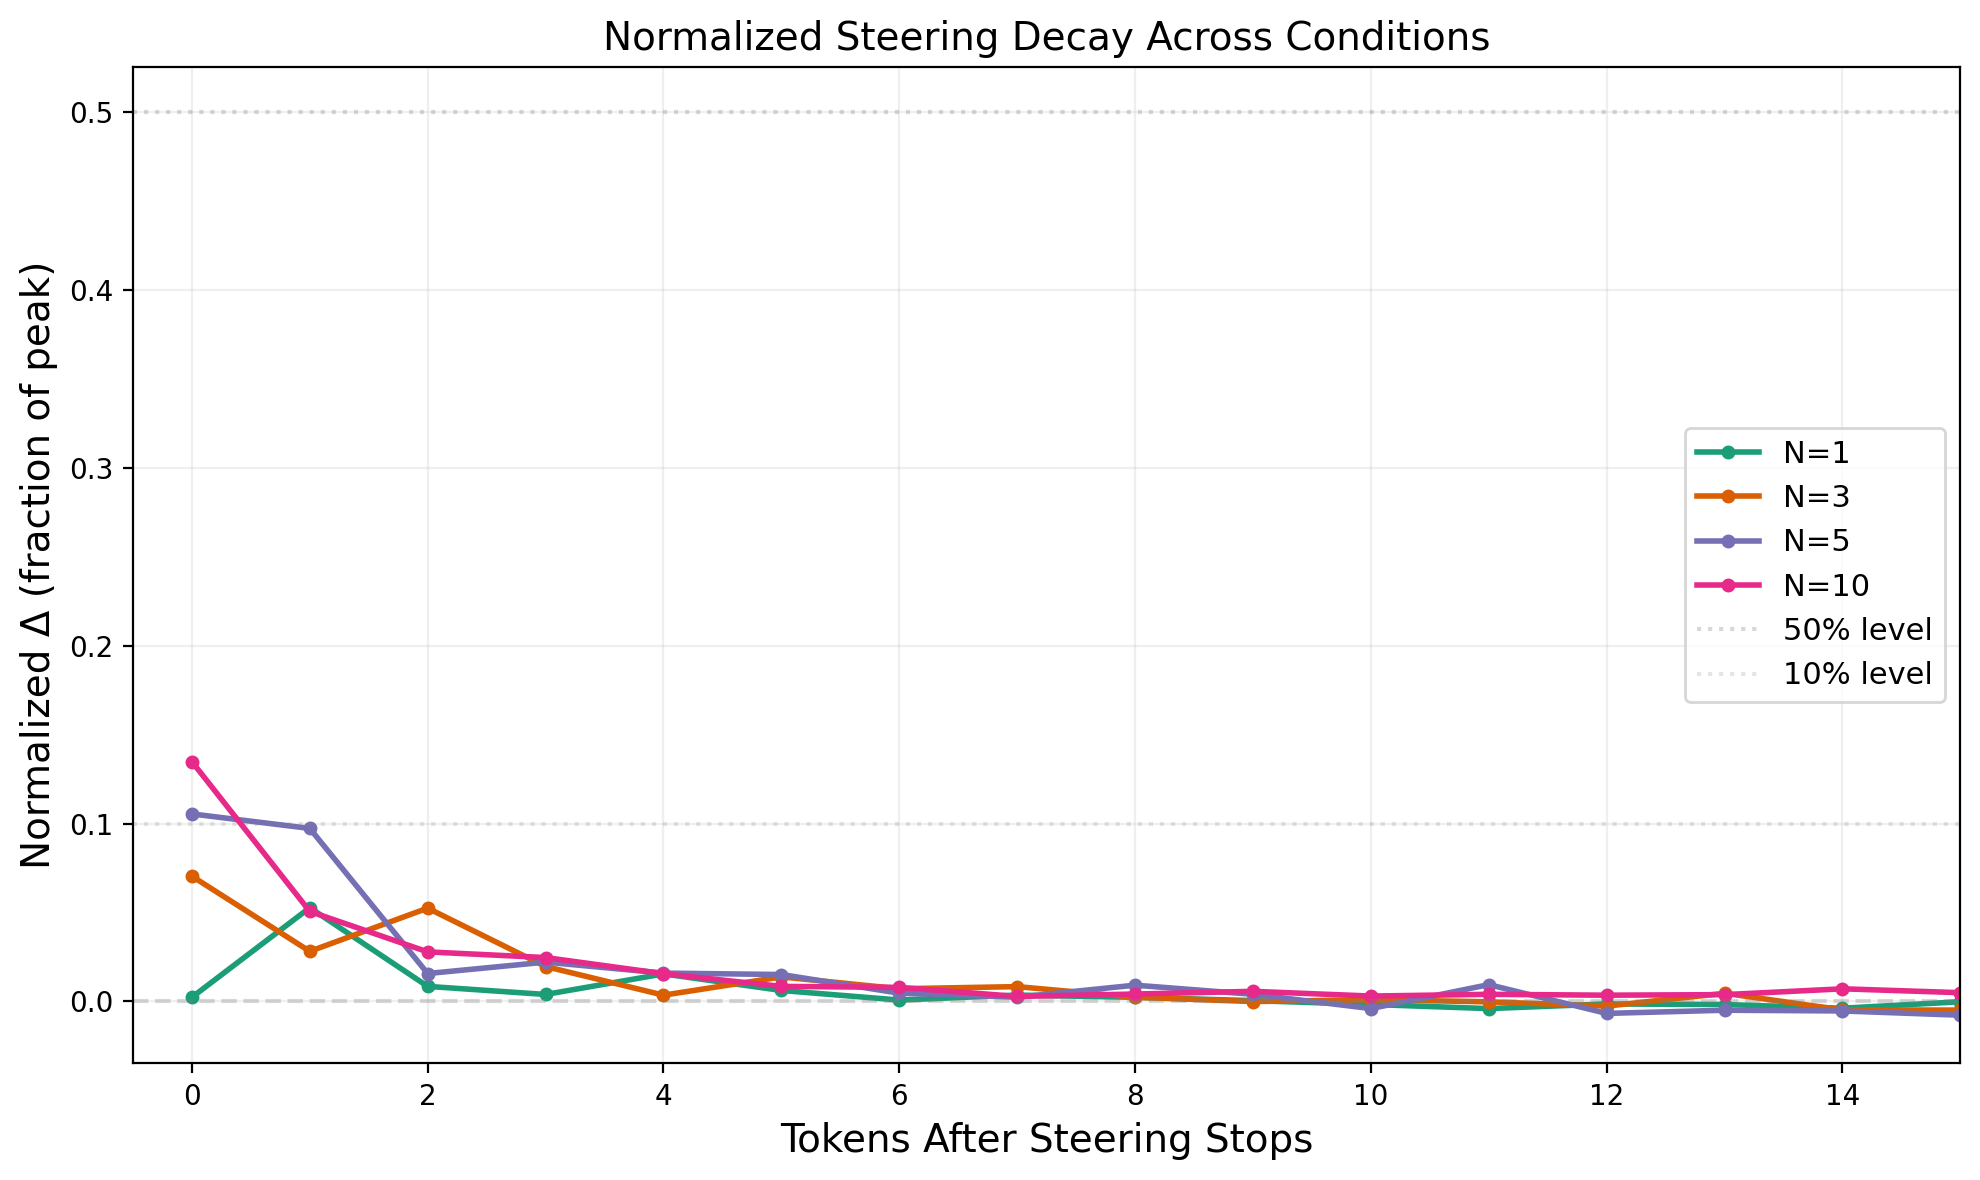
\includegraphics[width=0.95\linewidth]{figures/fig5_normalized_decay.png}
\caption{Normalized decay curves ($\deltaprojection / \deltaprojection^{\mathrm{peak}}$) for all initial-steering conditions. All curves drop below 10\% within 1--3 tokens after the steering vector is removed, confirming that near-instantaneous decay is robust across steering durations.}
\label{fig:normalized}
\end{figure}

\subsection{Free Generation}

\Figref{fig:free_gen} shows the $\deltaprojection$ curves under free (autoregressive) generation, where the model generates its own tokens after the initial steering window. These curves are substantially noisier than the teacher-forced conditions because different tokens at each step produce different activation patterns. The general trend---rapid decay followed by oscillation near zero---is consistent with the teacher-forced results, but the noise makes precise characterization difficult. This highlights why the controlled, teacher-forced experimental design is necessary for measuring decay dynamics.

\begin{figure}[t]
\centering
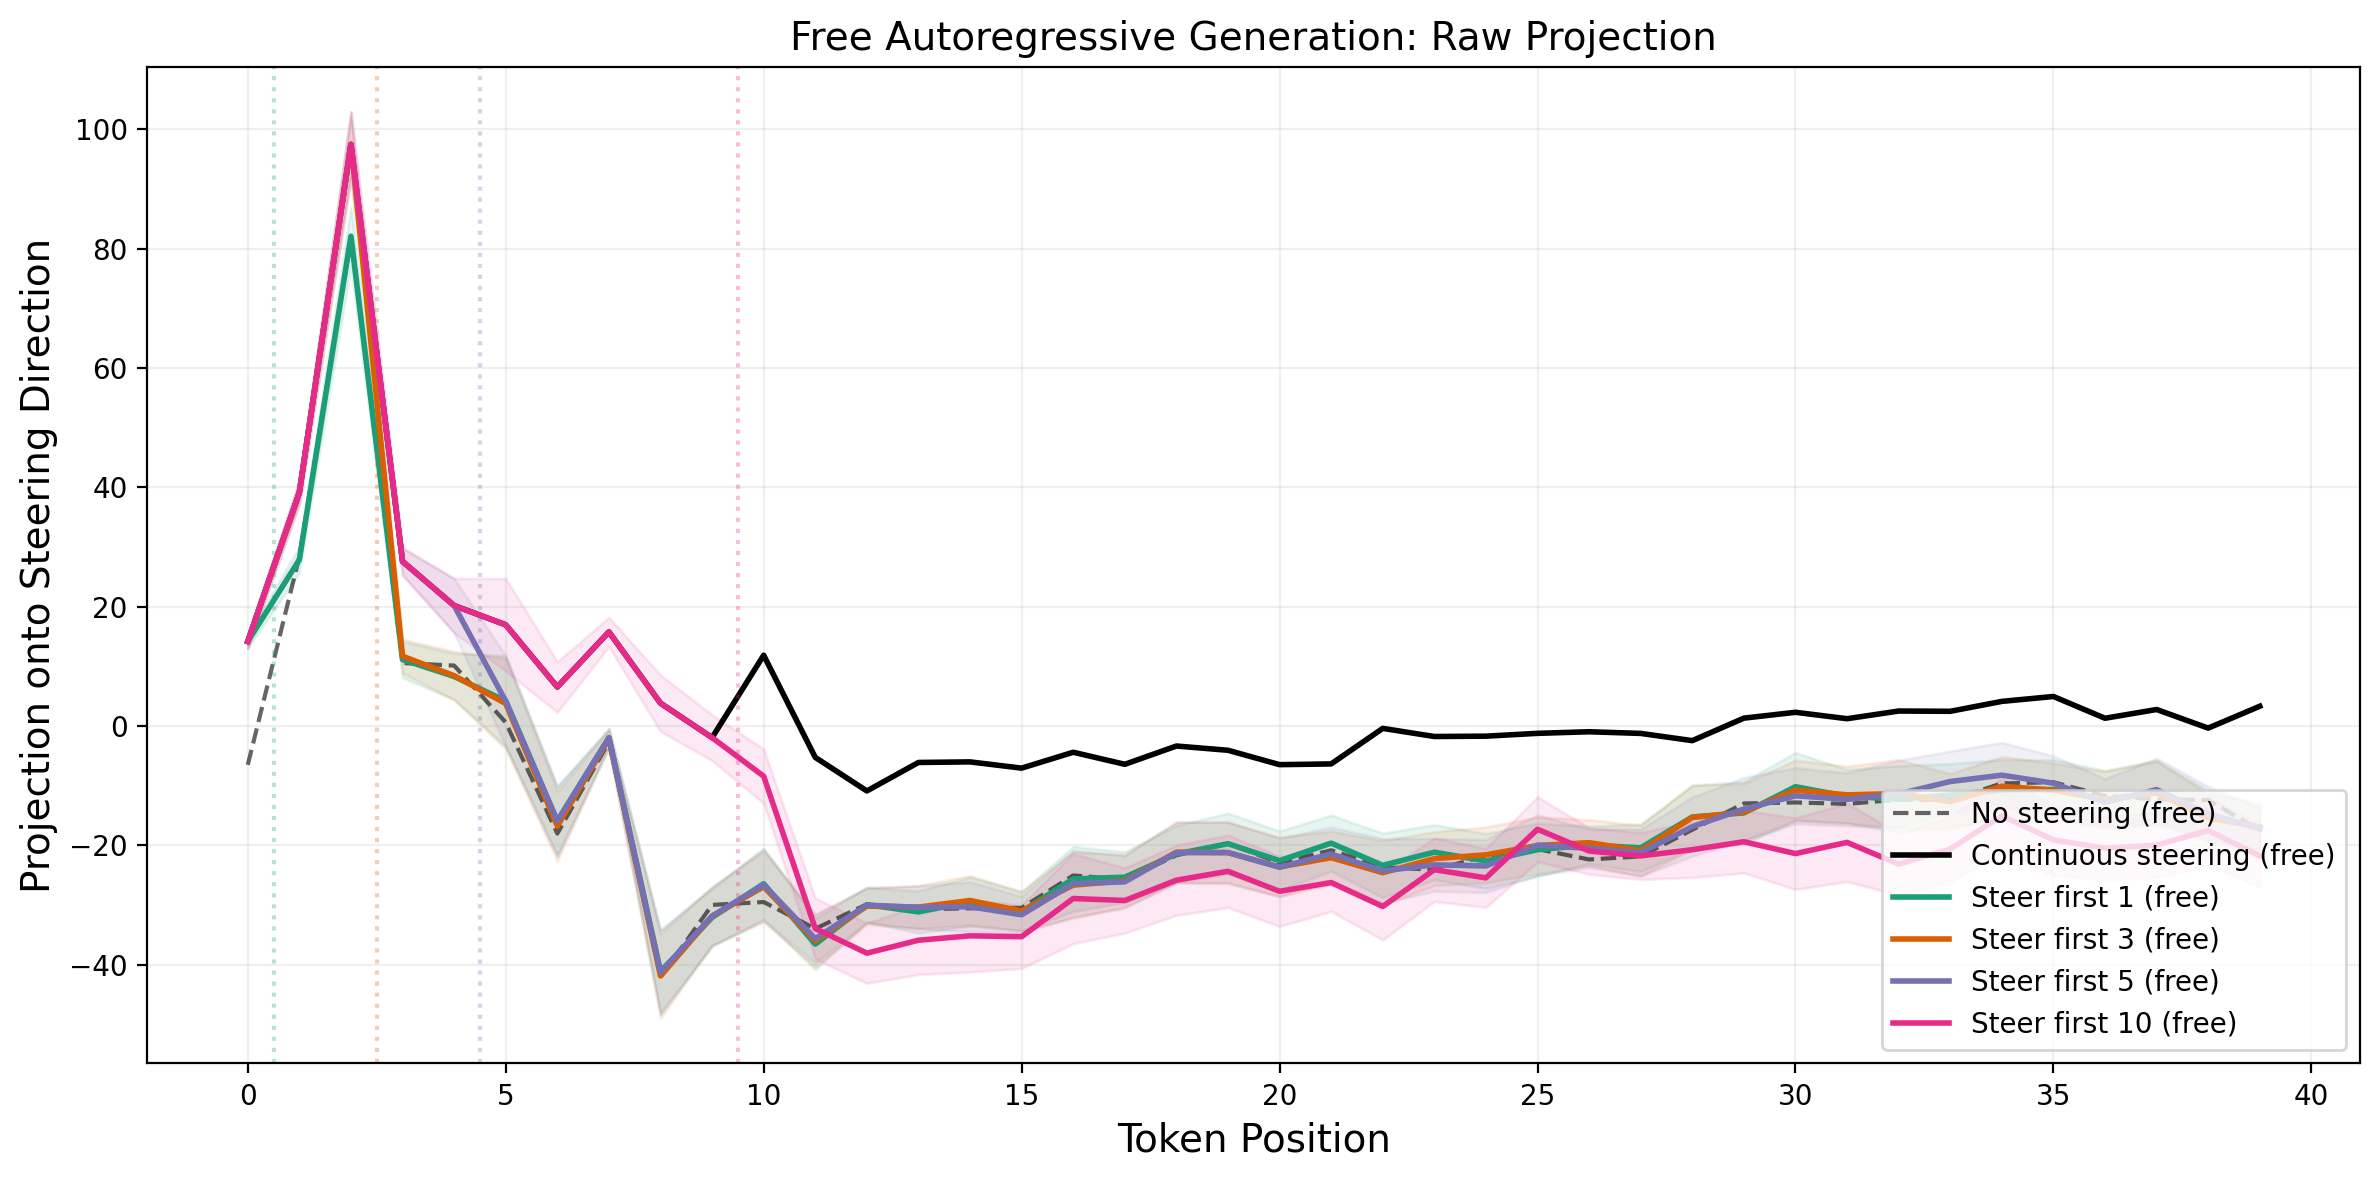
\includegraphics[width=0.95\linewidth]{figures/fig4_free_generation.png}
\caption{Steering projection under free autoregressive generation (no teacher-forcing). The signal is substantially noisier than teacher-forced conditions because token sequences diverge from baseline, producing different activation patterns at each step. The general trend of rapid decay is consistent with teacher-forced results.}
\label{fig:free_gen}
\end{figure}
